\documentclass{article}

\usepackage[poster]{staix_2026}

\usepackage[utf8]{inputenc}
\usepackage[T1]{fontenc}
\usepackage{hyperref}
\usepackage{url}
\usepackage{booktabs}
\usepackage{amsfonts}
\usepackage{microtype}
\usepackage{xcolor}
\usepackage{graphicx}
\usepackage{amsmath,amssymb,amsthm}

\title{A Statistical Audit of LLM Calibration Heterogeneity\\Across Knowledge Domains}

\author{%
  Anonymous Author 1 \\
  \texttt{anon1@anon.edu}
  \And
  Anonymous Author 2 \\
  \texttt{anon2@anon.edu}
}

\begin{document}

\maketitle

\begin{abstract}
LLM calibration is nearly always reported as an aggregate scalar, obscuring
where miscalibration concentrates. We develop a statistical audit framework
(three-level mixed-effects model, isotonic reliability curves,
Benjamini--Hochberg FDR) and apply it to MMLU across seven instruction-tuned
models from three families spanning six parameter scales. Subject-level ECE
rankings are highly correlated (Spearman $\rho \in [0.80, 0.94]$ across all
15 pairs of larger models), the same subjects are robustly worst- and
best-calibrated across models, and within Qwen the entropy coefficient on
the calibration gap grows monotonically with scale. The stability of these
patterns provides empirical motivation for subject-aware recalibration.
\end{abstract}

\section{Setup}
We extract token-level logprobs over A/B/C/D for all 14{,}042 MMLU
questions on GPT-4o-mini, Llama-3-8B-Instruct, and
Qwen-2.5-\{0.5B, 1.5B, 3B, 7B, 14B\}-Instruct. The outcome is the signed
calibration gap $\mathrm{gap}_i = c_i - y_i$ (max softmax confidence minus
correctness). A three-level mixed model
$\mathrm{gap}_{ijk} = \mu + \mathbf{x}_{ijk}^\top\boldsymbol{\beta}
+ u_k + v_{jk} + \varepsilon_{ijk}$ decomposes variance across questions,
subjects, and domains; per-subject gaps are tested with one-sample $t$-tests
and Benjamini--Hochberg FDR.

\section{Findings}

\paragraph{(i) Where calibration fails---and where it doesn't.}
Across the six larger models, \texttt{virology} and \texttt{professional\_law}
appear in the top-10 most miscalibrated for every model; a cluster of
college-level technical subjects (\texttt{abstract\_algebra},
\texttt{college\_mathematics}, \texttt{machine\_learning}) is in the top-5 for
four of six. Symmetrically, \texttt{marketing} and
\texttt{high\_school\_psychology} are in the bottom-10 for every model.
Specialization level tracks miscalibration: high-school subjects show
systematically smaller gaps than their college-level counterparts.

\paragraph{(ii) Cross-model and cross-family stability.}
All 15 pairwise Spearman correlations among the six larger models fall in
$[0.80, 0.94]$ (Figure~\ref{fig:heatmap}); cross-family GPT-4o-mini vs.\
Qwen-7B/14B at 0.92/0.91 is comparable to the strongest within-family pair
(Qwen-7B vs.\ Qwen-14B at 0.94). Qwen-0.5B is a conspicuous exception
($\rho \in [0.13, 0.20]$), driven by 10.6$\times$ positional bias toward the
D option---we read this as a lower bound below which our elicitation protocol
breaks down.

\paragraph{(iii) Within-Qwen scaling.}
Across four matched-precision Qwen checkpoints (1.5B fp16, 3B, 7B, 14B), the
entropy coefficient on the calibration gap grows monotonically
($-0.004 \to +0.006 \to +0.029 \to +0.040$, last two $p<0.001$): at 7B and
14B, confidence stays near saturation across the first three entropy
quartiles while accuracy still drops, so the gap widens on the model's
harder items (Q1 vs.\ Q4 gap: $+0.05$ vs.\ $+0.37$ at 7B; $+0.03$ vs.\
$+0.46$ at 14B). The between-subject ICC jumps from 1.5B to 3B
(0.017 $\to$ 0.051) and is essentially flat thereafter. This is consistent
with prior reports of RLHF-induced confidence saturation.

\begin{figure}[h]
  \centering
  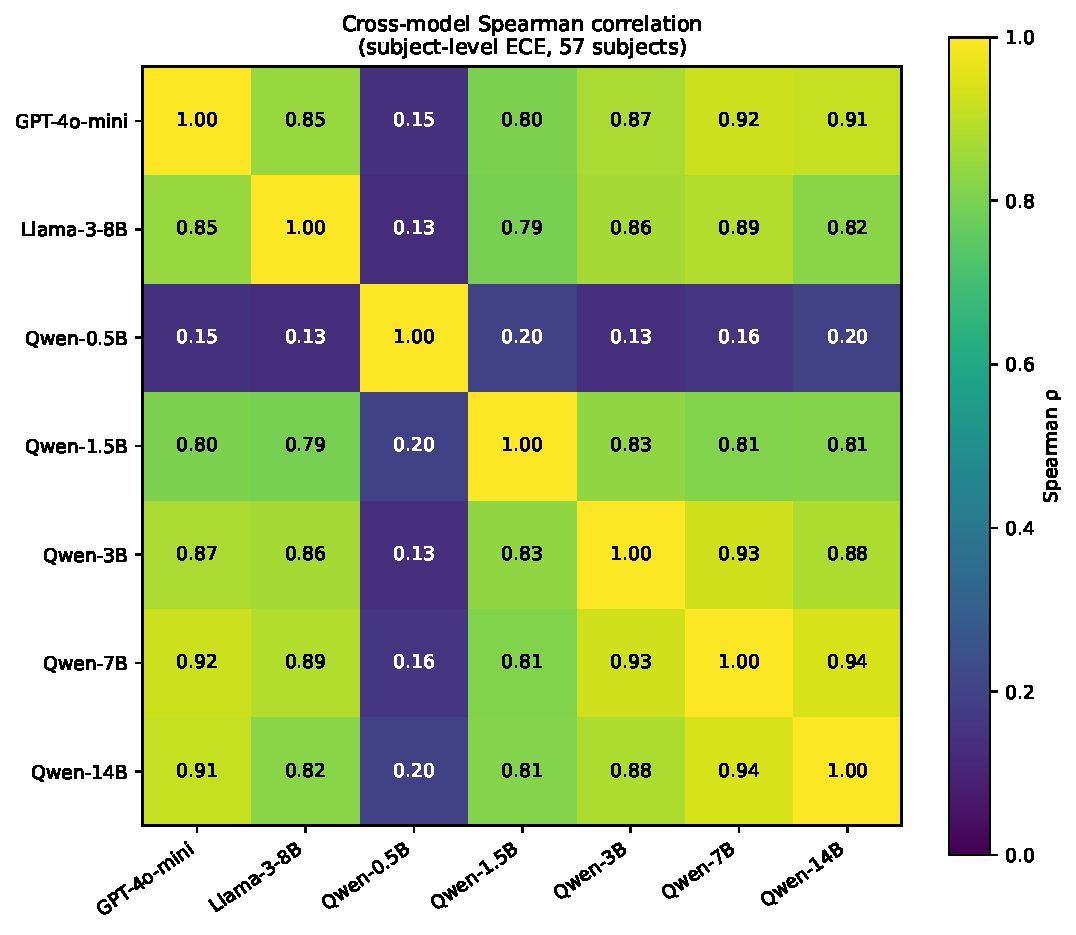
\includegraphics[width=0.55\textwidth]{figures/cross_model_heatmap_7m.pdf}
  \caption{Spearman rank correlation of subject-level ECE across the seven
  models (57 common subjects). Among the six larger models, all 15 pairwise
  correlations fall in $[0.80, 0.94]$. Qwen-0.5B's correlations with the
  others are $[0.13, 0.20]$, reflecting a qualitatively different
  miscalibration pattern driven by extreme positional bias.}
  \label{fig:heatmap}
\end{figure}

\section{Implications}
Cross-model stability is the precondition that makes subject-aware
recalibration worth scoping: a correction informed by one model's subject
rankings will generalize to others. A global recalibration would
under-correct the worst-calibrated cluster
(\texttt{professional\_law}, \texttt{virology}, college-level technical
content) while over-correcting subjects like \texttt{marketing}. The
robustly worst-calibrated subjects double as a transferable diagnostic for
flagging miscalibration on new models before deployment, without re-running
the full 57-subject audit.

\end{document}
